\myChapter{HSV and RGB comparison in Evolutionary Art}\label{chap:art}


\begin{flushright}{\slshape
    I've seen many things, my friend, but you're right:
    \\nothing quite as wonderful as the things you see.} \\ \medskip
    --- {The Doctor. Vincent and the Doctor. Doctor Who.}
\end{flushright}


\minitoc\mtcskip
\vfill




\lettrine{A}{s} part of the \textbf{Objective 4} (\objectiveresearch), in this chapter SOA-EA and OSGiLiath will be used to develop a SOEA. 

The research objective of this application is to study the differences % with respect to what? FERGU: añadido abajo
of using the information of the HSV (Hue, Saturation, Value) and RGB (Red,
Green, Blue) histograms in fitness function during the evolution. Although the two
histograms represent the same information, using HSV (instead as RGB)
as a color model increases the accuracy in image retrieval and
indexing, as explained by \person{Sebe and Lew}
\cite{COLORDIFFERENCES}.






 %A population
%of artistic works (individuals) are evaluated with an aesthetic
%measure to yield a score (fitness). These individuals are combined and
%mutated to generate an offspring with inherited properties of the
%parents, during a certain number of times. % until algo, ¿no? - JJ FERGU: quitado

% Esto es parte de una tesis y como tal tienes que tratarlo. ¿Por qué
% es interesante para la tesis este capítulo? ¿Qué parte de la tesis
% estás probando? - JJ FERGU: añadido



In this chapter, the {\em Processing} \cite{PROCESSING} framework is
integrated inside OSGiLiath % why? En una tesis hay que justificarlo
                            % TODO - JJ FERGU: 
to take advantage of the capabilities offered in image manipulation and analysis. 
{\em Processing} services are then used  to model the
individuals, generate their associate images and extract information
of them (HSV, RGB and Average histograms) to fit with the histograms
of the test images.

% Pero ¿cuál es el objetivo de este trabajo? El objetivo no es evaluar
% arte generativo, porque no se ha aportado nada en ese tema o no está
% claro qué vas a aportar. Es demostrar lo fácil que es adaptar
% Osgiliath a un nuevo problema, midiendo la velocidad de desarrollo y
% ejecución y uso de nuevos entornos como el dichoso processing - JJ FERGU: reescribiendo para que esté relacionado con la tesis


\section{Background}

Evolutionary Art \cite{EART} is a branch of generative art \cite{PHEROGRAPHY}, which is created using a
computer, following the principle of the survival of the fittest, 
using Evolutionary Computation methods.

Metrics such as opinion from humans or image characteristics (for
example, specific combination of colours) can be used to score the
generated images. %We will adopt the latter in this chapter, % why? - JJ
%whose  

%The results of this investigation can help in
%future evolutionary art algorithms, adding the most appropiate color
%model feature with other features available in the literature. For
%example, to be used as one of the features of any kind of
%classifier. % En una tesis el trabajo futuro no viene a cuento. Tienes
            % que evaluar el trabajo de por sí. - JJ FERGU: tienes razón
Computational Aesthetics ``is the research of computational
methods that can make applicable aesthetics decisions in a similar
fashion as humans can'' \cite{COMPAESTH}. In the field of
computational aesthetics, evolutionary systems can play an important
role, by enabling the evolution of aesthetically pleasing or
innovative structures \cite{dipaola2009incorporating}. Evolutionary % y te interesa meterlo como parte de la tesis porque... - JJ
art is characterized by the use of evolutionary principles and natural
selection as a generative process. One of the earliest applications of
evolutionary systems to generate art is the proposal of \person{Sims}
to use an EA to create complex images \cite{sims1991artificial} or
virtual creatures  \cite{sims1994evolving}. In evolutionary art
systems, the evaluation of the aesthetics can be done using human
feedback, with some interactive evaluation of the population, such as
\cite{ashlock2006evolutionary,draves2006electric,moroni2000vox} and
\cite{sims1991artificial}. It also can be achieved by using an
automatic evaluation of fitness, as presented in
\cite{aguilar2008robotic,den2010comparing,dipaola2009incorporating,li2012investigating},
and \cite{sims1994evolving}. % Si lo que quieres hacer es aportar algo
                             % en arte evolutivo, tienes que tomártelo
                             % un poco más en serio, evaluando
                             % artísticamente los resultados,
                             % seleccionando las fotos originales,
                             % buscando arte generativo a base de
                             % bolas similar... No te despistes de tu
                             % objetivo que es el de la tesis - JJ FERGU: tienes razón, esto es qeu lo hicimos entre todos en el hackathon

One of the main challenges in Evolutionary Art is how to measure
aesthetic value of the generated pieces. The source of this difficulty
lies in the inherent complexity, subjectivity and dynamism of
aesthetics. Nevertheless, a wide number of metrics has been
presented. According to \person{Galanter}
\cite{galanter2012computational}, these measures can be classified
into several categories in several pieces of research. The first
category involves the evaluation of the aesthetics of a piece of art
by a formula or principle (e.g., pythagorean proportions). Other
measures apply certain principles of design, such as the rule of
thirds or color theory (e.g., using complimentary colors in Pop Art in
the work of \person{den Heijer and Eiben} \cite{den2012evolving}),
neural networks or complexity measures.   % ¿Cuál vas a usar? No se
                                % trata de hacer "name dropping",
                                % tienes que mencionar lo que sea
                                % interesante o incumba a tu tesis - JJ FERGU: quitadas las morrallas

%This classification also provides a sub-classification for
%evolutionary systems. If aesthetical evaluation is done by human it is
%called {\em interactive} evolutionary systems. Another category is
%performance % utility, más que performance - JJ
% based goals: certain properties of the art piece are evaluated and
% optimized based on performance measures (e.g., usable surface in a
% furniture design generator). Other systems use an exemplar (i.e.,
% real world example) as a way to measure the fitness of the
% individuals. % esto más que arte es diseño, no confundas. Además,
              % ¿cómo se llama esta subclase si la de antes es
              % interactiva? - JJ FERGU: quitando todo
 %Finally, some models use the idea that the complexity is directly
 %related to aesthetics and follow the path firstly stablished in
 %\cite{birkhoff2003aesthetic}.  Given the multidimensional nature of
 %aesthetics judgement, multi-objective EAs are a straightforward
 %option to deal with this multidimensionality. %¿Es lo que vas a usar?
                                %Si no, es que no estás usando lo
                                %"mejor" para tu tesis. - JJ
 %Other extensions to EA, like coevolution or agent swarm behavior, can
 %be used in evolutionary art systems. % ¿Eso es una subclasificación?
                                % ¿Cómo se usan? Una tesis no es un
                                % gran ejercicio de "name dropping",
                                % justifica cosas con enlaces,
                                % intégralas en la narrativa de tu
                                % tesus y sobre todo añade citas. Por
                                % cierto, agent swarm no es una
                                % extensión de EAS- jj FERGU: to fuera

%A brief classification of the aesthetic measures found in the
%evolutionary art systems mentioned in the previous paragraph % NO ESTÁ
                                % EN EL PREVIO, SINO EN EL
                                % ANTERIOR. ¿Por qué no lo pones ahí?
                                % - JJ
% is shown in Table~\ref{table_class}.


%\begin{SCtable}[][t]

%\resizebox{11cm}{!}{
%\begin{tabular}{p{4cm}p{7cm}}
%\hline
%\rowcolor{colorCorporativoSuave}Type & Aesthetic Measure \\ \hline \hline
%\rowcolor{colorCorporativoMasSuave}Formulaic and Geometric Theories & Fractal dimension \cite{den2010comparing}, Image order \cite{li2012investigating}, Benford Law \cite{del2005benford}\\ \hline
%\rowcolor{colorCorporativoSuave}Based on Design Principles &  Color contrast (hue) \cite{den2012evolving},  Color ingredient \cite{li2012investigating}, Composition, tonality and color \cite{dipaola2009incorporating}.\\ \hline
%\rowcolor{colorCorporativoMasSuave}Interactive Evolutionary Computation & The electric sheep project \cite{draves2006electric} \cite{ashlock2006evolutionary,moroni2000vox}\\ \hline
%\rowcolor{colorCorporativoSuave}Error relative to Exemplars &  Resemblance score \cite{dipaola2009incorporating}, pixel comparation \cite{aguilar2008robotic}\\ \hline
%\rowcolor{colorCorporativoMasSuave}Performance based goals & Evolving virtual creatures \cite{sims1994evolving} \\\hline
%\rowcolor{colorCorporativoSuave}Complexity measures & Image complexity \cite{li2012investigating}, Machado and Cardoso aesthetic measure \cite{machado1998computing}\\ \hline
%\end{tabular}
%}
%\caption{Classification of the aesthetic measures used in a brief review of the literature on evolutive art.} 
%\label{table_class} 
%\end{SCtable}

%Several methods for the representation of the art in evolutionary
%art % the _art_ in evolutionary _art_? Seriously? - JJ
% have been proposed. In symbolic expression, the genotype is a tree of
% expressions and the phenotype consists in the image produced  by the
% evaluation of the tree. Shape grammars can also be used as a formal
% description of the image. Previously existing images can be used as a
% basis for the evolution process. Finally, other representations can
% be based on mathematical models, like fractals or cellular
% automata. % Esto ¿a santo de qué? ¿Qué tiene que ver con las
           % clasificaciones? - JJ FERGU: to fuera!


%\rowcolors{2}{gray!25}{white}


% Sin dedicarle una línea a enlazar tu trabajo con el trabajo
% anterior, ni hablar de clasificación, ni de representación, ni de
% por qué avanza el estado del arte ni tu tesis, venga, vamos a hablar
% de processing. Una tesis es una narrativa continua. Aquí el lector
% ya se ha perdido y no entiende a qué viene a cuento toda la parte
% expositiva del capítulo anterior - JJ FERGU: reescribiendo capítulo entero y movido de sitio


%\section{Histograms} % ¿lo ves como antes no hablabas de histogramas? - JJ FERGU: cambiado de sitio

In this chapter, the histogram feature will be used as aesthetic measure.
The color histograms of 
the images represent the frequency of occurrence of each color
intensities present in the image, by accounting for such sharing
pixels color intensity values. % ¿ein? ¿Google translator? - JJ FERGU: puede ser, porque esto lo escribimos entre varios y a mí no me suena...

The histogram is composed of different ranges or bins that represent a value or set of values of color intensity. % si esto es parte o traslación literal del trabajo, deberías reescribirlo (vas a tener que hacerlo de todas formas para integrarlo con la tesis) - JJ
 The color space is defined as a model representation with respect to color intensity values. Two color models are used in this chapter: RGB (Red, Green, Blue) and HSV (Hue, Saturation and Value). The RGB model is an additive color model in which red, green and blue are added together in different proportions to reproduce a wide range of colors, while the HSV is based on hue or tone, saturation and brightness. While the RGB model is the closest to the way color is processed in some machines, the HSV representation provides a more accurate way to model how humans perceive colors, and also provides more information in image retrieval \cite{COLORDIFFERENCES}.
Figure \ref{fig:histogram} shows the RGB histogram of the image in Figure \ref{fig:flevopark}.

\begin{SCfigure}[20][htb]
\centering
   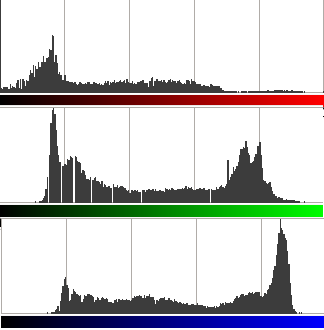
\includegraphics[scale =0.6] {gfx/art/histogram.png}
\caption{RGB histogram of Figure \ref{fig:flevopark}. }
\label{fig:histogram}
\end{SCfigure}

\begin{SCfigure}[20][htb]
\centering
   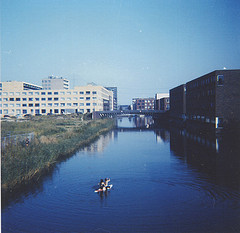
\includegraphics[scale =3] {gfx/art/flevopark.jpg}
\caption{Test image to compare with the Fitness functions of our algorithm.}
\label{fig:flevopark}
\end{SCfigure}


\section{Applying SOA-EA}
\label{sec:art:soaea}

Once the background has been provided, SOA-EA will be applied.

\subsection{Identification}

The problem to solve with this SOEA is to generate images that match the most to a given . Therefore infrastructure services to read, write and analyze images will be needed. In the problem domain, it is required an {\em Initializer} that generates individuals with the coded information of an image, and a {\em FitnessCalculator} to obtain a fitness of equality with the example image. Finally, in the Algorihm Domain a Mutation specific for this kind of individuals will be created. 

%Drawer (individual)
%ArtisticMutation
%ArtisticFitnessCalculator


\subsection{Specification}

The input of the services are implementations of the {\em Individual} class that codify the information of each generated image. The {\em ListIndividual}   implementation previously defined will be used: the genome of the individual is a list of
{\em primitives}. % ¿El genoma es una lista para llevar a cabo los experimentos? ¿En serio? - JJ FERGU: borrado
Each primitive has a position, size and color. This list can
be recombined or mutated (changing the color, position or radium of a
primitive of the list). 


% hala, una subsección con una sola frase. ¿Por qué se
                     % usa esto? ¿Cómo lo enlazas con la literatura?
                     % ¿Fue lo primero que se te ocurrió? ¿Por qué
                     % usas círculos y no cuadrados? ¿O círculos y
                     % cuadrados? ¿O divisiones fractales? ¿O, en
                     % general, cualquier otra cosa? - JJ FERGU: quitada subsección


For this piece of research, we focused on the aesthetics measure of
histogram comparison. The fitness functions are included in the
``Error relative to Exemplars'' category, using \person{Galanter}
\cite{galanter2012computational} classification. The idea is to obtain
an image with the same proportion of tones and colors of a 
existent image. 

% Y eso ¿por qué tendría algo que ver con los valores
                % estéticos de la imagen? Hasta ahora no has
                % justificado que el histograma tenga nada que ver con
                % lo bonita que es - JJ

Three different fitness functions will be implemented in three different services:
\begin{itemize}
\item {\em RGBFitnessCalculator}: The difference of the RGB histogram of the individual with the RGB histogram of the test image.
\item {\em HSVFitness}: The difference of the HSV histogram of the individual with the HSV histogram of the test image.
\item {\em AverageFitness}: An average of the two previous differences (uses the previous two services).
\end{itemize}

The range of the these fitness function has been normalized to vary from 0 (totally different histograms) to 1 (the same histogram).

For every color property (i.e., RED, GREEN, BLUE, HUE, SATURATION and VALUE), the histogram is computed using the expression (\ref{eq:histogram}) for each possible value (0-255). Then, again for every property, the difference between the target image and the individual histograms is obtained using (\ref{eq:diff}). Finally, the three fitness are calculated: RGB fitness (\ref{eq:RGB}), HSV fitness (\ref{eq:HSV}) and AVERAGE fitness (\ref{eq:AVERAGE}).

\begin{eqnarray}
  \label{eq:histogram}
  H(c, prop) = \frac{1}{N}\sum_{j=0}^N \left\{\begin{matrix}
1 & prop(j) = c\\ 
0 & otherwise
\end{matrix}\right. \\
\label{eq:diff}
diff(h_1, h_2) = \sum_{j=0}^{255} |h_1(j) - h_2(j)|
\end{eqnarray}
\begin{eqnarray}
  d_R(i) = diff(H(i, RED), H(target, RED))\\
  d_G(i) = diff(H(i, GREEN), H(target, GREEN))\\
  d_B(i) =  diff(H(i, BLUE), H(target, BLUE))\\
  \label{eq:RGB}
  fitness_{RGB}(i) = 1 - 128\frac{d_R(i) + d_G(i) + d_B(i)}{3}
\end{eqnarray}
\begin{eqnarray}
  d_H(i) = diff(H(i, HUE), H(target, HUE))\\
  d_S(i) = diff(H(i, SAT), H(target, SAT))\\
  d_V(i) =  diff(H(i, VAL), H(target, VAL))\\
  \label{eq:HSV}
  fitness_{HSV}(i) = 1 - 128\frac{d_H(i) + d_S(i) + d_V(i)}{3}
\end{eqnarray}
\begin{eqnarray}
  \label{eq:AVERAGE}
  fitness_{AVERAGE}(i) = \frac{fitness_{RGB}+fitness_{HSV}}{2}
\end{eqnarray}




\subsection{Implementation and deployment}



To draw the information contained in the individuals, the {\em Processing} framework has been chosen.
\footnote{\url{http://www.processing.org/}}.  %¿Dónde has justificado el uso de histogramas? Tampoco engañes
      %al lector: Una cosa es Processing y otra los histogramas. Si
      %estamos a processing, estamos a processing - JJ FERGU: reestructurado
 {\em Processing} \cite{PROCESSING} is a framework formed by a simple
 programming language and an integrated development environment (IDE)
 (shown in Figure \ref{fig:ideProc}) primarily created for electronic
 and visual artists such as designers, musicians. This framework has been chosen because it offers
 the following advantages: % No se usa etc en lenguaje formal. Y esto
                           % os lo he dicho en más de mil papers - JJ FERGU: quitados

%\begin{itemize}
%\item Processing was created for artists, rather than programmers. So, it allows very complex drawings and interactive applications with few lines of code.
%\item It is an Open Source software (licensed under the GNU Lesser General Public License), and counts with a large development community.
%\item It is based on OpenGL, thus providing 3D acceleration.
%\item It also includes more than 100 libraries for video, sound, physics, computer vision and networking.
%\item Easy integration with Java, HTML5 and Android.
%\end{itemize}

%Lo que estás haciendo es dibujar bolas. las ventajas de processing no
%tienes qu emedirlas de forma absoluta, sino relativa a usar
%simplemente JS con el canvas. En todo caso, siempre se trata de
%ventajas para la tesis. Deja el modo "justificar lo que se me
%ocurrió" y entra en el modo "justificar la tesis" - JJ FERGU: quitado

\begin{SCfigure}[htb]
\centering

%\subfigure[Processing IDE]{
   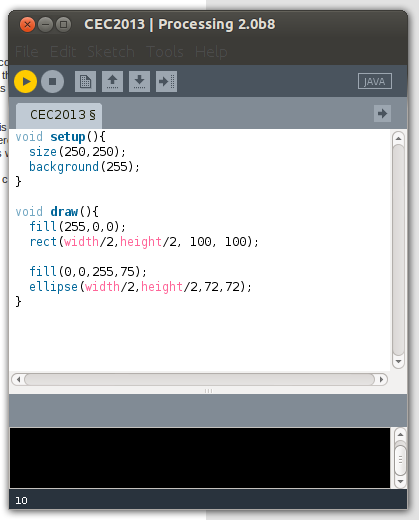
\includegraphics[scale =0.55] {gfx/art/Processing.png}
%   \label{fig:subide}
% }
%\subfigure[Runtime of the code.]{
   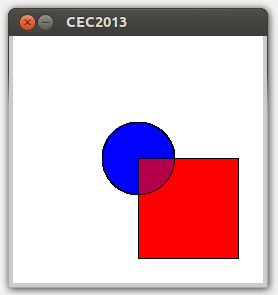
\includegraphics[scale =0.45] {gfx/art/run.png}
%   \label{fig:subsketch}
% }

\label{fig:ideProc}
\caption{Processing IDE and sketch execution. }
\end{SCfigure}

%However, being a light framework, there exist some disadvantages:
%\begin{itemize}
%\item More complex applications require more programming skills.
%\item The calculations of large computer images are a bit inefficient (although expert programmers can manage OpenGL at low level to fix this).
%\end{itemize} FERGU: esto también lo quito

There exist a lot of interactive artistic projects made with
Processing; examples include art generation, artificial life,
interactive music and other. A good selection can be seen in
\url{http://processing.org/exhibition/}. % Aquí podías citar los
                                % fireworks que hicimos con leonardo
                                % Trujillo - JJ

%Processing is composed by several modules: %En general, cualquier
                                %itemización es mala. Y más cuando,
                                %como esta, suena a copy paste. ¿En
                                %serio que saber que processing tiene
                                %un módulo de tipografía es
                                %interesante para tu tesis? - JJ FERGU: tienes razón, quitado

%\begin{itemize}
%\item Structure: Includes typical programming functions as is the case of return, draw, void, and everything related to the structure of the program.
%\item Environment: Formed by the functions that handle the modeling of the window: cursor, width, height, background, for example.
%\item Data: formed by the data types that make up the different program variables (int, char, float).
%\item Control: Consisting in relations operators.
%\item Shape: it is formed by all functions of the treatment of figures 3D and 2D.
%\item Input: input interactivity features such as functions for the mouse, keyboard or files.
%\item Output: output interactivity features such as write on the screen, save the image or serial control.
%\item Transform: transformations such as rotations or translations.
%\item Lights and Cameras: Functions for the treatment of the lights and cameras.
%\item Color: Functions to handle color of the figures.
%\item Image: Functions for loading images or textures.
%\item Rendering: Functions for rendering images.
%\item Typography: Functions for dealing with text.
%\item Math: Functions for dealing with all mathematical functionality.
%\end{itemize}

{\em Processing} % usa alguna tipografía para diferenciar processing la librería de processing el verbo - JJ FERGU: hecho
can be integrated with Java just by adding a {\em jar} (a
Java library) to existing software.

A new {\em bundle} called OSGiLiART has been
added to the publicly-available source code of OSGiLiath \footnote{\url{https://github.com/fergunet/osgiliath/tree/master/OSGiLiART}}.  % URL - JJ FERGU: Done
Then, using the packages available in the {\em Processing} library an algorithm can generate individuals, manipulate images or extract information. The service {\em Drawer} has been implemented with  {\em ProcessingDrawer}). To create random individuals we have implemented the {\em ArtisticInitializer} to generate individuals composed by the primitives in {\em Processing}. The implementation {\em ArtisticMutator} modifies randomly one of the elements of the individual. Finally, several {\em FitnessCalculator} implementations have been added: {\em HSVFitnessCalculator}, {\em RGBFitnessCalculator} and {\em AverageHistogramFitnessCalculator}. There is not necessary to modify other existent service implementations (such as existent {\em Recombinators} or {\em Replacers} explained in previous chapters), because the abstract design of OSGiLiath.





%\noindent This section shows how Processing has been used in the EA,
%the individual representation, the fitness functions, and the
%parameters of the experiments. % Una tesis debe ser también una metodología. ¿Esta metodología coincide con la del resto de los capítulos? - JJ FERGU: quitado










\section{Experimental Results}
\label{sec:results}

A steady-state evolutionary algorithm has been used. % ¿Por qué? ¿No
                                % es Osgiliath tan flexible? ¿Por qué
                                % no pruebas 7 tipos diferentes?
                                % Tienes que demostrar que conoces los
                                % algoritmos subyacentes.
% A partir de aquí paso de decirte que justifiques cada decisión
% individual. UNA TESIS ES UNA TESIS. Tienes que justificar todo, y
% quiero decir todo (estoy viendo desde aquí la tasa de crossover, por
% ejemplo) en función de tu conocimiento del estado del arte y la
% metodología que estés proponiendo en la tesis.
Each individual is randomly generated at the initialization of the EA. The genome size is 50 elements (circles of maximum radium of 128 pixels). Population size has been set to 32 individuals. Uniform crossover rate is 0.5, and a binary tournament has been chosen for selection (that is, a pool of 16 parents is selected and crossed). Mutation probability is 0.04 (the usual value of {\em 1/genomesize}). Finally, the image size for each individual is 256x256 pixels. The individuals have been compared with the histograms obtained from the image of Figure \ref{fig:flevopark} to guide the evolution. 

 Because of the stochastic nature of the EAs, each algorithm
has been executed 30 times for each different fitness formula. Table
\ref{tab:results} shows the average differences (and standard
deviation) attained with each fitness used. As can be seen, using the
HSV histogram differences as fitness produces a higher RGB similarity
(and therefore, average) than using the RGB or Average
fitness. However, using the average between the two histogram
differences produces higher similarity in HSV (0.294) than only taking
into account the HSV. The maximum fitness is around 25\% of similarity
with the original image since the individual is a list of 50 circles,
and therefore, only a maximum of 50 different colors are used (while
in the original jpg image can be more than millions). See the
histogram of a generated best individual by the algorithm in Figure
\ref{fig:histoind}. An example of evolution for each fitness can be
seen in Figure \ref{fig:rgbgens}, \ref{fig:hsvgens} and
\ref{fig:averagegens}. Comparing with the RGB histogram as fitness, a
bigger fluctuation in the HSV is produced (Figure
\ref{fig:rgbgens}). This can be explained because the RGB information
tends to be more noisy than HSV information: in fact, in
\cite{COLORDIFFERENCES} authors explain the problems this histogram
offers with respect to HSV in image retrieval. Although there is the
same information modeled in both histograms, the transformation from
one to another is not linear, so there is no relation with the
histograms of individuals generated during the evolution. 

\begin{SCtable}[][t]
\resizebox{11cm}{!}{
\begin{tabular}{ccccc}
\hline
\rowcolor{colorCorporativoSuave}Differences used  in Fitness & Obtained RGB      & Obtained HSV  & Obtained Average \\ \hline \hline
\rowcolor{colorCorporativoMasSuave}RGB Histogram    & 0.267 $\pm$ 0.012	& 0.170 $\pm$ 0.010 	& 0.218 $\pm$ 0.009	\\ \hline
\rowcolor{colorCorporativoSuave}HSV Histogram    & 0.227 $\pm$ 0.017	& 0.265 $\pm$ 0.021	& 0.246 $\pm$ 0.010 \\ \hline
\rowcolor{colorCorporativoMasSuave}Average Histogram& 0.173 $\pm$ 0.012	& 0.294 $\pm$ 0.013	& 0.234 $\pm$ 0.010 \\ \hline
\end{tabular}
}
\caption{Results for the different fitness (average of the 30 executions and standard deviation). Only one histogram type is used for fitness calculation, but the other values obtained are also added.}
\label{tab:results}
\end{SCtable}

\begin{SCfigure}[20][htb]
\centering
   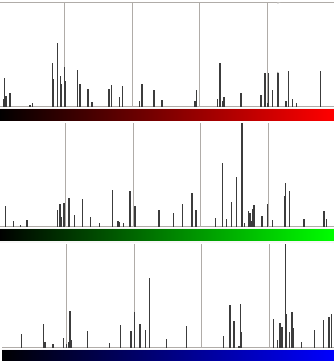
\includegraphics[scale =0.6] {gfx/art/individuohist.png}
\caption{RGB histogram of a solution generated by the algorithm.}
\label{fig:histoind}
\end{SCfigure}

\begin{SCfigure}[20][htb]
   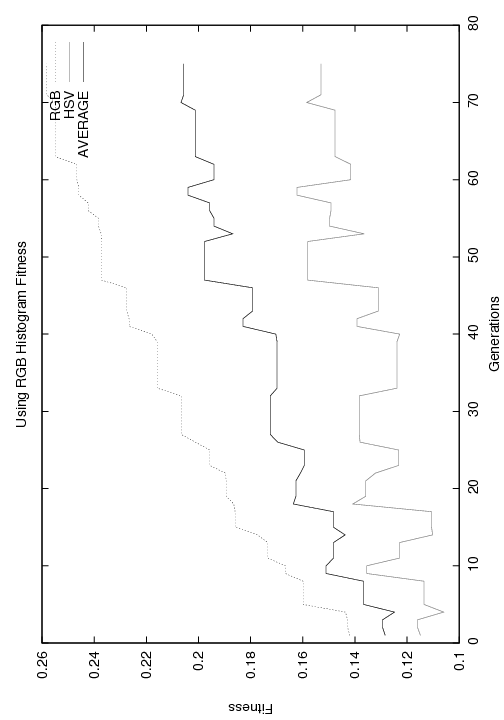
\includegraphics[angle=-90,scale =0.40] {gfx/art/rgbgens.png}
\caption{Evolution of the difference in RGB histogram of the best individual compared with the test image. }
\label{fig:rgbgens}
\end{SCfigure}

\begin{SCfigure}[20][htb]
   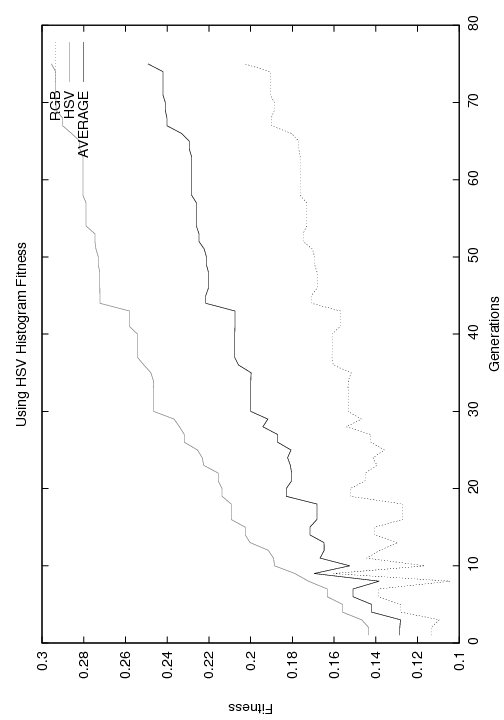
\includegraphics[angle=-90,scale =0.40] {gfx/art/hsvgens.png}
\caption{Evolution of the difference in HSV histogram of the best individual compared with the test image. }
\label{fig:hsvgens}
\end{SCfigure}

\begin{SCfigure}[20][htb]
   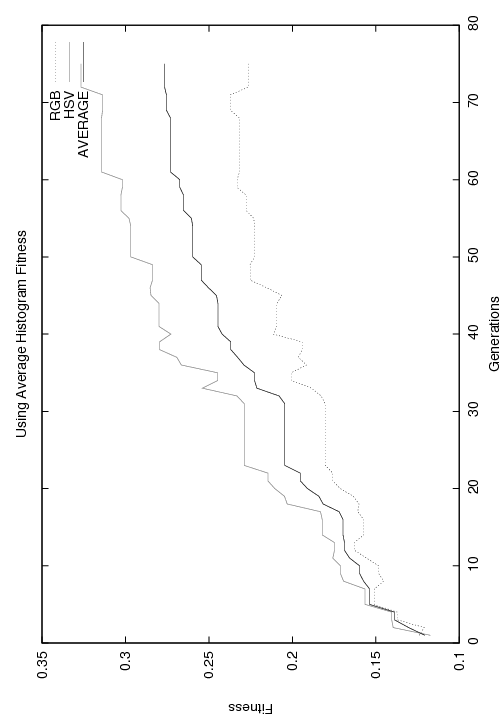
\includegraphics[angle=-90,scale =0.40] {gfx/art/averagegens.png}
\caption{Evolution of the difference of average of RGB and HSV histogram of the best individual compared with the test image. }
\label{fig:averagegens}
\end{SCfigure}

The best individuals obtained are shown in Figure
\ref{fig:bestinds}. Note that, although the numeric fitness is
similar, they produce different color tones. This can be explained for
the limitation of colors used in the individual representation, as
previously said, or the noisy characteristic of the RGB
histogram. Figure \ref{fig:collage} shows one evolution of the best
individual using the HSV fitness in the first 64 generations. %Estás
                                %hablando de evolución "estética" y de
                                %arte generativo. ¿No deberías
                                %comentar algo del valor artístico de
                                %lo obtenido? - JJ

\begin{SCfigure}[20][htb]
\centering
%\subfigure[Best individual using RGB]{
   
\includegraphics[scale =0.5] {gfx/art/RGB.png}
 %}
%\subfigure[Best individual using HSV]{
   
\includegraphics[scale =0.5] {gfx/art/HSV.png}
 %}
%\subfigure[Best individual using AVERAGE]{
   
\includegraphics[scale =0.5] {gfx/art/AVERAGE.png}
 %}
\caption{Best individuals obtained with the three fitness used (HSV, RGB and AVERAGE).}
\label{fig:bestinds}
\end{SCfigure}

\begin{SCfigure}[20][htb]
   
\includegraphics[scale =0.10] {gfx/art/collage.png}
\caption{Evolution of the best individual using the HSV histogram difference. }
\label{fig:collage}
\end{SCfigure}

\section{Conclusions and Future Work}
\label{sec:conclusions}
In this chapter {\em Processing} has been integrated in OSGiLiath
to create an Evolutionary Algorithm  to generate images and to extract
image information using HSV and RGB histograms. This complies the Objective 4 (\objectiveresearch) of this thesis.

 % .. y esto me ha
                                % servido en esta tesis para probar x
                                % o y - JJ
Individuals are represented as a list of Processing primitives
(circles) and the fitness functions used are based on the similarity
with an existent aesthetic image. % como yo propongo en mi tesis en x
                                % o y - JJ
 Three different fitness functions services
using color histogram have been tested: difference between the HSV and
RGB histograms, and an average difference of the two histograms at the
same time. Experiments show that better results in terms of similarity
are obtained using the HSV comparison (due to the noisy information
provided by the RGB).  % y por lo tanto esto implica para mi tesis x o
                       % y. 

% Una tesis no incluye trabajo futuro salvo en las conclusiones - JJ FERGU: quitado
%The future work for this research also includes more experiment with other kind of individuals, apart from circles: using other primitives, such as rectangles or triangles, for example. The use of textures and gradients will generate images with higher number of colors, obtaining more fidelity (more than 25\%) with the test image. Other metrics explained in previous sections will be also implemented. Finally, our intention is not only to create only static images, but use the Processing libraries to create evolutionary interactive art combining sounds and motion. 

%More complex measurements will be studied in next works, taking into
%account that the HSV is the color mode that provides more information
%during the evolution, having less noisy behaviour.

% Esto canta a inclusión a capón de un artículo en una tesis con la
% que tiene en común solo el software usado. O lo adaptas muy mucho en
% la línea que te he puesto en los comentarios o lo suprimes - JJ FERGU: exactamente era eso lo que había hecho, pero me lo revisaste antes de que lo adaptara más a la tesis. Tengo que adaptarlo más a la tesis, OJO!!!!